\section*{Appendix}
The appendix is organized as follows:
\begin{itemize}
\item In \autoref{sec:app-add_results}, we present additional plots to supplement the experiments from the main paper:
\begin{itemize}
    \item In \ref{sec:app-motivation}, we replicate \Cref{fig:motivation} across models (LLaDA, Dream) and datasets (GSM8k, MATH).
    \item In \ref{sec:app-dream}, we replicate \Cref{fig:combined-results} for policies trained on Dream.
    \item In \ref{sec:app-alpha}, we show results for the same setting as \autoref{fig:gsm8k-bl32-llada} and \autoref{fig:math500-bl32-llada} but with a denser $\alpha$-grid.
    \item In \ref{sec:app-policy_temp}, we plot the impact of varying the policy temperature $\tau_{\pi}$.
    \item In \ref{subsec:appendix-model-transfer}, we provide model transfer results for the MATH dataset.
    \item In \ref{subsec:appendix-length-transfer}, we provide generation length (L) transfer results for the MATH dataset.
 \end{itemize}
\item In \autoref{sec:appendix_config}, we  provide implementation and hyperparameters details.
\item In \autoref{sec:appendix-dpls}, we describe dynamic Plackett-Luce sampling as an alternative to Bernoulli sampling.
\item In \autoref{sec:appendix-es}, we detail our \emph{expert steering} approach.
\item In \autoref{sec:appendix_extended_background} we discuss an extended background discussion on discrete diffusion models, to benefit readers who are not familiar with this paradigm.

\end{itemize}

\newpage

\section{Additional Results}
\label{sec:app-add_results}

\subsection{\autoref{fig:motivation} replicated for \{\textsc{LLaDA-8B-Instruct, Dream-7b-Instruct}\} $\times$ 
\{\textsc{GSM8k, MATH-500}\}}
\label{sec:app-motivation}
\begin{figure}[htbp]
    \centering
    
\includegraphics[width=0.8\textwidth]{new_plots_nov4/fig1/simple-fig1-llada-gsm8k_legend.pdf}
    
    \vspace{0.5em}
    
    \begin{subfigure}[b]{0.4\textwidth}
        \centering
        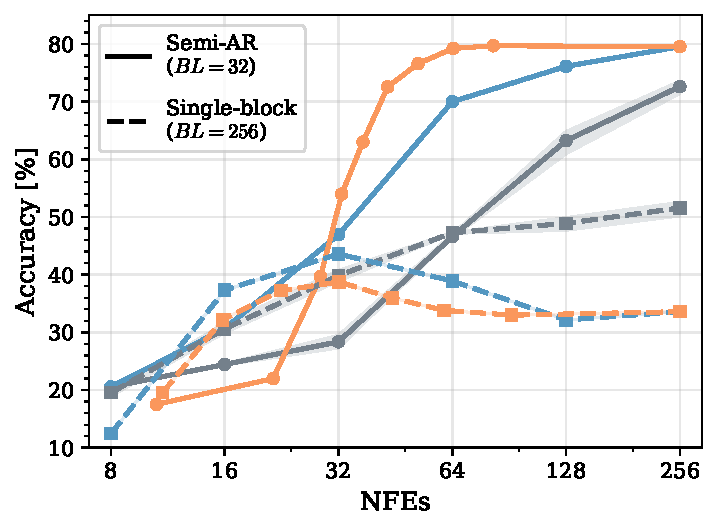
\includegraphics[width=\textwidth]{new_plots_nov4/fig1/simple-fig1-llada-gsm8k.pdf}
        \caption{LLaDA on GSM8k}
        \label{fig:llada-gsm8k}
    \end{subfigure}
    \begin{subfigure}[b]{0.4\textwidth}
        \centering
        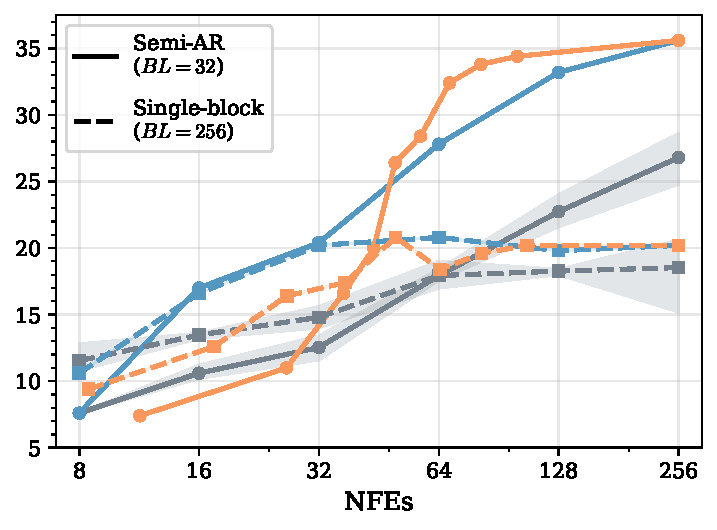
\includegraphics[width=\textwidth]{new_plots_nov4/fig1/simple-fig1-llada-math.pdf}
        \caption{LLaDA on MATH-500}
        \label{fig:llada-math}
    \end{subfigure}
    
    \vspace{0.5em}
    
    \begin{subfigure}[b]{0.4\textwidth}
        \centering
        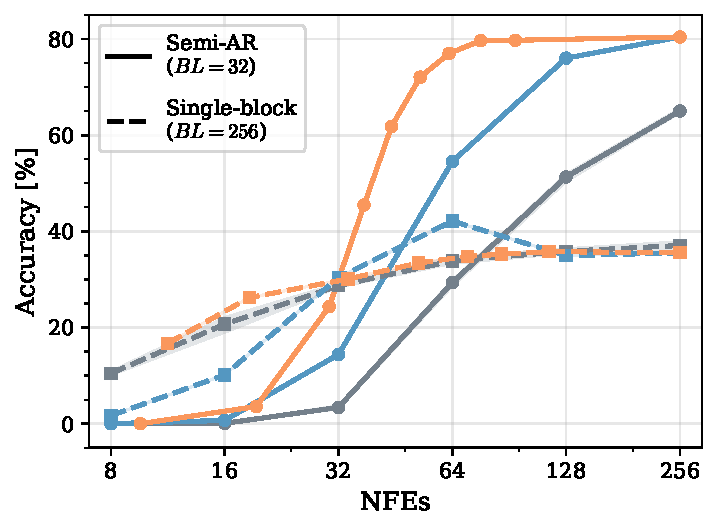
\includegraphics[width=\textwidth]{new_plots_nov4/fig1/simple-fig1-dream-gsm8k.pdf}
        \caption{Dream on GSM8k}
        \label{fig:dream-gsm8k}
    \end{subfigure}
    \begin{subfigure}[b]{0.4\textwidth}
        \centering
        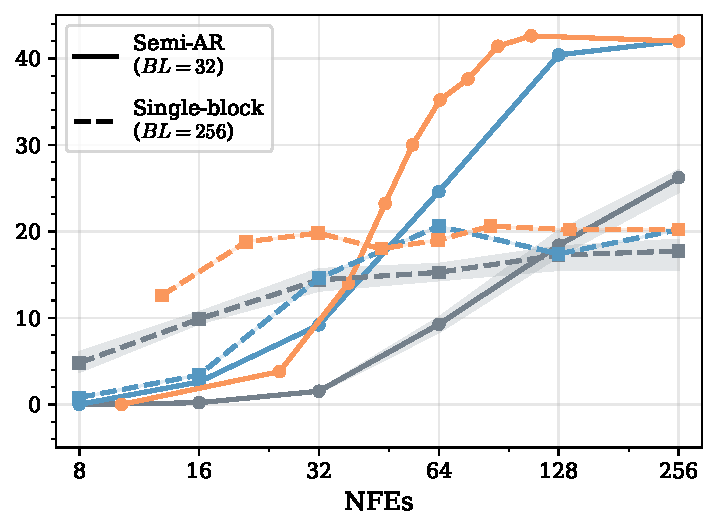
\includegraphics[width=\textwidth]{new_plots_nov4/fig1/simple-fig1-dream-math.pdf}
        \caption{Dream on MATH-500}
        \label{fig:dream-math}
    \end{subfigure}
    
    \caption{Performance comparison with ($BL=32$; \protect\solidline) and without ($BL=256$; \protect\dashedline) semi-AR generation. The same trend observed in \Cref{fig:motivation} holds across all models and datasets: confidence-based heuristics perform well under semi-AR generation but degrade significantly without it.
    }
\end{figure}

\newpage
\subsection{\autoref{fig:combined-results} replicated for \textsc{Dream-7b-Instruct}}
\label{sec:app-dream}

\begin{figure}[ht]
    \centering
    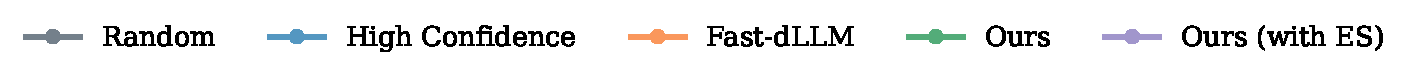
\includegraphics[width=0.95\textwidth]{new_plots_nov4/legends/fig3.pdf}

    \vspace{0.3cm}

    \begin{subfigure}[t]{0.24\textwidth}
        \centering
        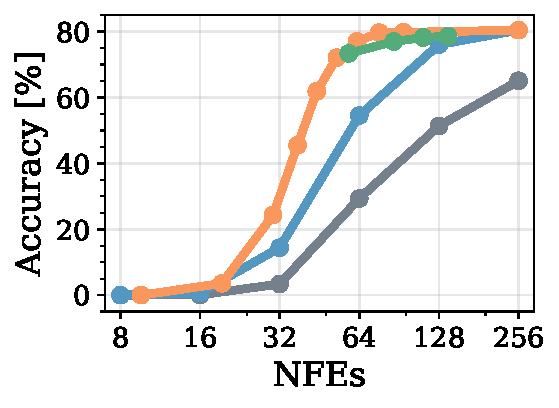
\includegraphics[width=\textwidth]{new_plots_nov4/bl32/bl32-dream-gsm8k-temp0.5.pdf}
        \caption{GSM8k, $BL=32$}
        \label{fig:gsm8k-bl32-dream}
    \end{subfigure}
    \hfill
     \begin{subfigure}[t]{0.24\textwidth}
        \centering
        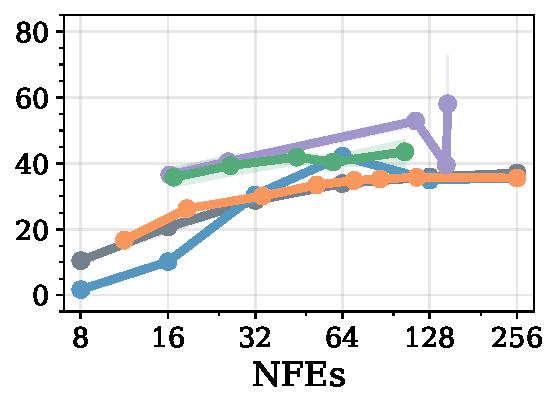
\includegraphics[width=\textwidth]{new_plots_nov4/bl256/bl256-with-wwfdd-dream-gsm8k-temp1.0-bernoulli.pdf}
        \caption{GSM8k, $BL=256$}
        \label{fig:gsm8k-bl256-dream}
    \end{subfigure}
    \hfill
    \begin{subfigure}[t]{0.24\textwidth}
        \centering
        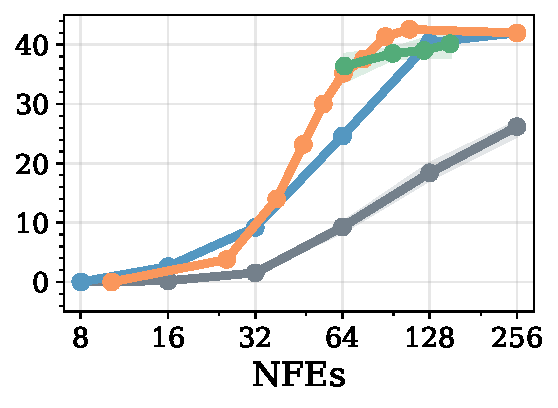
\includegraphics[width=\textwidth]{new_plots_nov4/bl32/bl32-dream-math-temp0.5.pdf}
        \caption{MATH-500, $BL=32$}
        \label{fig:math500-bl32-dream}
    \end{subfigure}
    \hfill
    \begin{subfigure}[t]{0.24\textwidth}
        \centering
        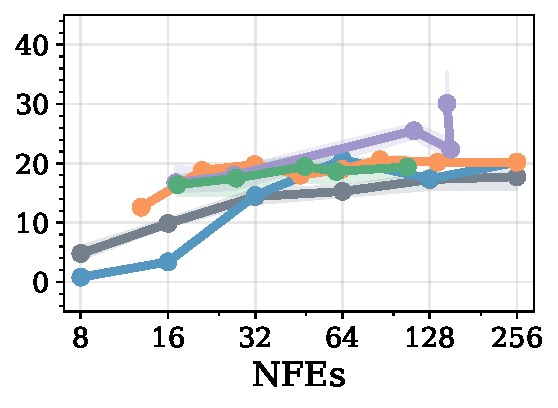
\includegraphics[width=\textwidth]{new_plots_nov4/bl256/bl256-with-wwfdd-dream-math-temp1.0-bernoulli.pdf}
        \caption{MATH-500, $BL=256$}
        \label{fig:math500-bl256-dream}
    \end{subfigure}

      \caption{Results for Dream in semi-AR (\Cref{fig:gsm8k-bl32-dream} \& \Cref{fig:math500-bl32-dream}) and full-diffusion (\Cref{fig:gsm8k-bl256-dream} \& \Cref{fig:math500-bl256-dream}) generation regimes. For the policies we vary $\alpha \in \{10, 3, 1, 0.3, 0 \}$ and use $\tau_{\pi}=0.5$ for $BL=32$ and $\tau_{\pi} = 1$ for $BL=256$. Unlike for LLaDA, where the learned policies clearly match Fast-dLLM in the mid-to-high NFEs regime for semi-AR generation, a small gap appears to remain for Dream. Furthermore, we found that the $\alpha = 10$ policy did not converge in the $BL=32$ setting when using Dream as the underlying language model (downstream accuracy thus not shown in (a), (c), to reduce clutter in the figures). Meanwhile, in the full-diffusion setting we do observe some performance gains, but here too they are smaller than were seen for LLaDA.}
    \label{fig:combined-results-dream}
\end{figure}

\subsection{Finer grid for $\alpha$}
\label{sec:app-alpha}

\begin{figure}[h!]
    \centering
    
\includegraphics[width=0.8\textwidth]{new_plots_nov4/legends/fig9.pdf}

    \vspace{0.3cm}

    \begin{subfigure}[b]{0.4\textwidth}
        \centering
        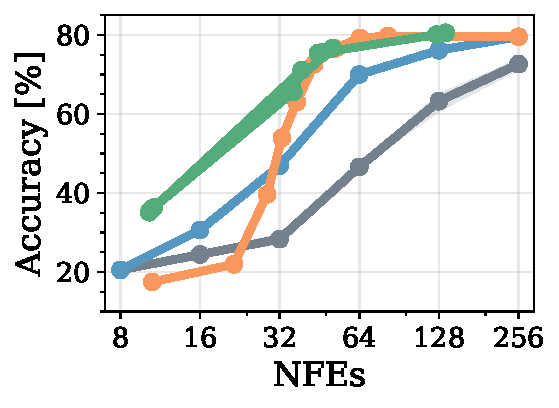
\includegraphics[width=\textwidth]{new_plots_nov4/ablation-denser-alpha/bl32-denser-llada-gsm8k-temp0.5.pdf}
        \caption{GSM8k, $BL=32$}
    \end{subfigure}
    \begin{subfigure}[b]{0.4\textwidth}
        \centering
        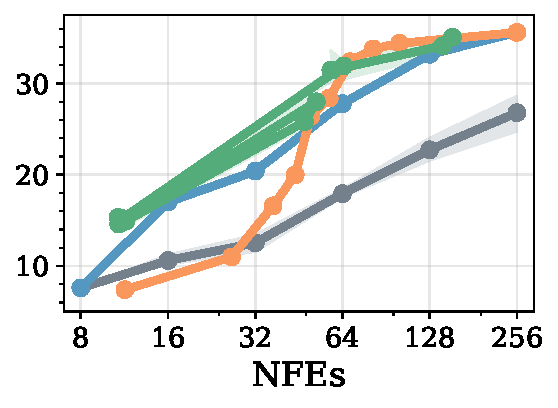
\includegraphics[width=\textwidth]{new_plots_nov4/ablation-denser-alpha/bl32-denser-llada-math-temp0.5.pdf}
        \caption{MATH-500, $BL=32$}
    \end{subfigure}
    \caption{$BL=32$ results for LLaDA with a denser regularization grid, $\alpha \in 
    \{10.0, 9.0, \ldots, 1.0, 0.3, 0.0\}$. Single training seed due to cost; error bars show (min, max) over three test-time seeds. Note that for $\alpha \geq 4.0$, the change in NFEs is not monotonic; different values lead to convergence either close to the $\alpha = 3.0$ policy, or to that of $\alpha =10.0$.}
    \label{fig:denser-alpha}
\end{figure}

\newpage
\subsection{Impact of policy temperature $\tau_{\pi}$}
\label{sec:app-policy_temp}

\begin{figure}[h!]
    \centering

    \vspace{0.3cm}
    
    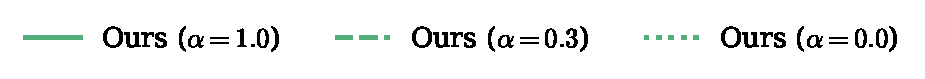
\includegraphics[width=0.66\textwidth]{new_plots_nov4/legends/fig8.pdf}

    \begin{subfigure}[b]{0.4\textwidth}
        \centering
        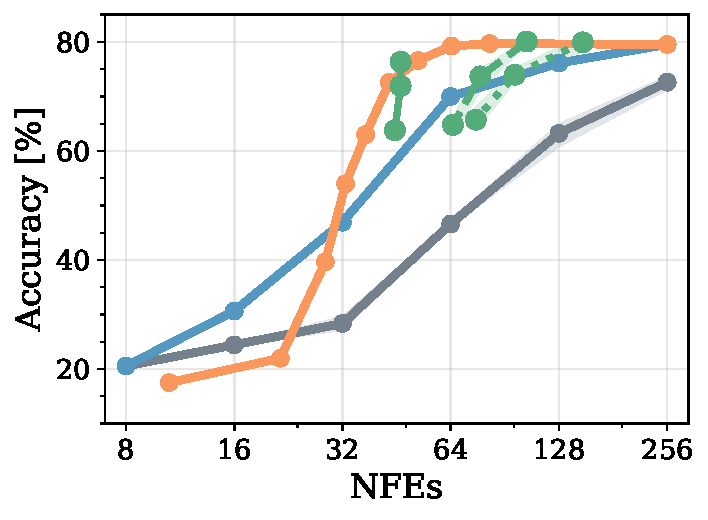
\includegraphics[width=\textwidth]{new_plots_nov4/alt-pareto/bl32-alt-llada-gsm8k.pdf}
        \caption{GSM8k, $BL=32$}
        \label{fig:gsm8k-bl32-alt-llada}
    \end{subfigure}
    \begin{subfigure}[b]{0.4\textwidth}
        \centering
        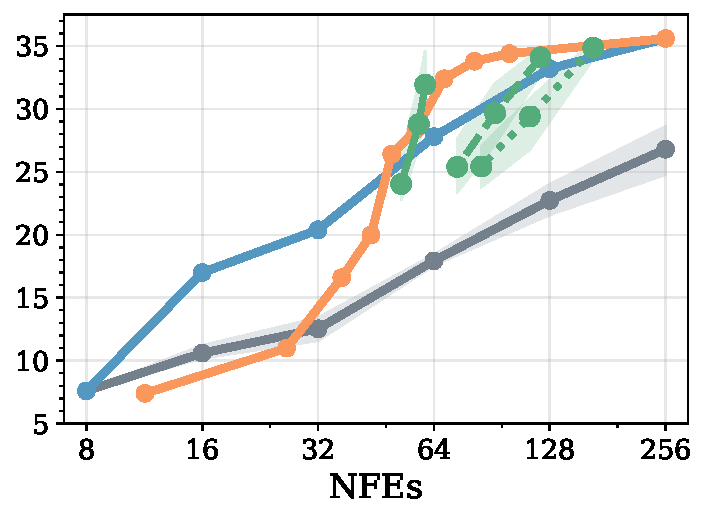
\includegraphics[width=\textwidth]{new_plots_nov4/alt-pareto/bl32-alt-llada-math.pdf}
        \caption{MATH-500, $BL=32$}
        \label{fig:math500-bl32-alt-llada}
    \end{subfigure}

    \vspace{0.5cm}

    \begin{subfigure}[b]{0.4\textwidth}
        \centering
        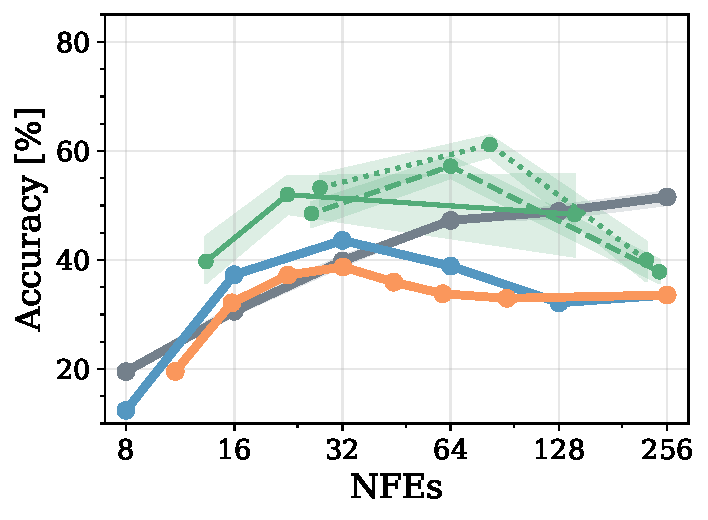
\includegraphics[width=\textwidth]{new_plots_nov4/alt-pareto/bl256-alt-llada-gsm8k.pdf}
        \caption{GSM8k, $BL=256$}
        \label{fig:gsm8k-bl256-alt-llada}
    \end{subfigure}
    \begin{subfigure}[b]{0.4\textwidth}
        \centering
        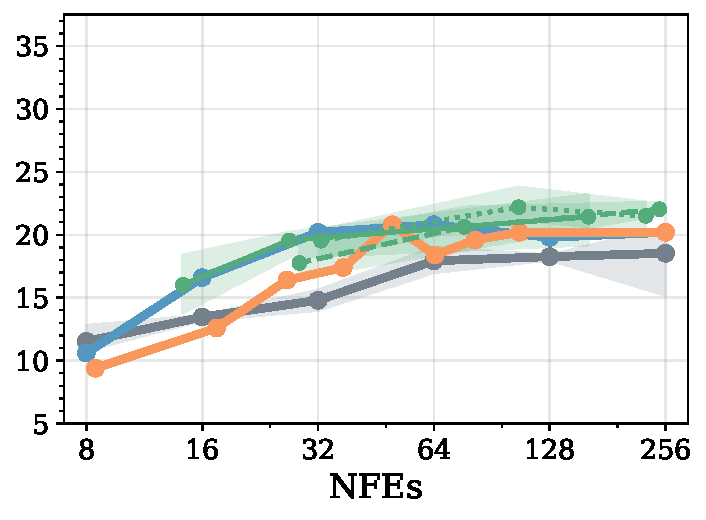
\includegraphics[width=\textwidth]{new_plots_nov4/alt-pareto/bl256-alt-llada-math.pdf}
        \caption{MATH-500, $BL=256$}
        \label{fig:math500-bl256-alt-llada}
    \end{subfigure}
    \caption{We study the effect of changing the policy temperature $\tau_{\pi}$ (cf. \Cref{sec:methods_policy}). For each $\alpha \in {3, 0.3, 0}$, we construct a corresponding test-time Pareto frontier by varying $\tau_{\pi} \in {1.5, 1.0, 0.5}$. Interestingly, in some cases—such as $\alpha = 0$ with $BL=32$—adjusting $\tau_{\pi}$ enables an effective trade-off between compute and performance. Moreover, we find that $\tau_{\pi} = 0.5$ is optimal in the semi-AR, while $\tau_{\pi} = 1$ performs best in the non-semi-AR ($BL=256$) setting.} 
    \label{fig:bl32-test-time-temp}
\end{figure}





\newpage

\subsection{Model transfer results}
\label{subsec:appendix-model-transfer}

\begin{figure}[h!]
    \centering
    
\includegraphics[width=0.8\textwidth]{new_plots_nov4/legends/fig9.pdf}

    \vspace{0.3cm}

    \begin{subfigure}[b]{0.4\textwidth}
        \centering
        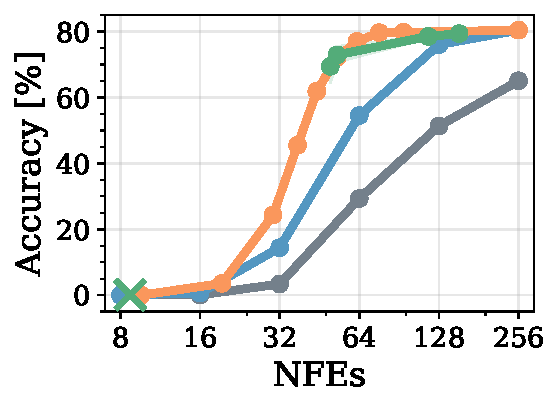
\includegraphics[width=\textwidth]{new_plots_nov4/model-transfer/llada-to-dream-bl32-gsm8k-temp0.5.pdf}
        \caption{GSM8k, $BL=32$}
    \end{subfigure}
    \begin{subfigure}[b]{0.4\textwidth}
        \centering
        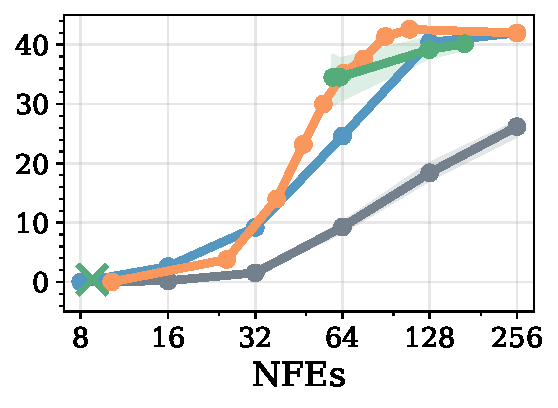
\includegraphics[width=\textwidth]{new_plots_nov4/model-transfer/llada-to-dream-bl32-math-temp0.5.pdf}
        \caption{MATH-500, $BL=32$}
    \end{subfigure}
    \caption{Model transfer results. We use policies trained on LLaDA and evaluate them on Dream with $\tau_{\pi} = 0.5$. Encouragingly, transferred policies give almost identical results compared to training Dream specific policies (cf. \Cref{fig:gsm8k-bl32-dream} \& \Cref{fig:math500-bl32-dream}). Note that the $\alpha=10$ policy is represented separately by a (\protect\scalerel*{\usebox{\boxgreen}}{\square}) in the lower left  to avoid misleading visualization when interpolating to $\alpha=3$.}
    \label{fig:model-transfer}
\end{figure}

\subsection{Sequence-length transferability}
\label{subsec:appendix-length-transfer}

\begin{figure}[h!]
    \centering
    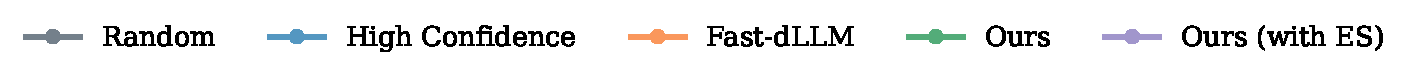
\includegraphics[width=\textwidth]{new_plots_nov4/legends/fig3.pdf}

    \vspace{0.3cm}

    \begin{subfigure}[b]{0.4\textwidth}
        \centering
        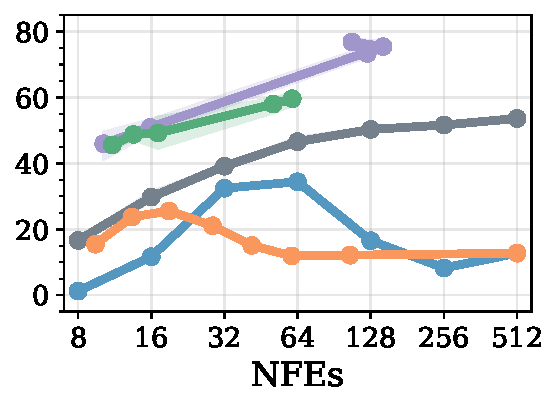
\includegraphics[width=\textwidth]{new_plots_nov4/length-transfer/bl256-to-bl512-llada-gsm8k-temp1.0.pdf}
        \caption{GSM8k}
    \end{subfigure}
    \begin{subfigure}[b]{0.4\textwidth}
        \centering
        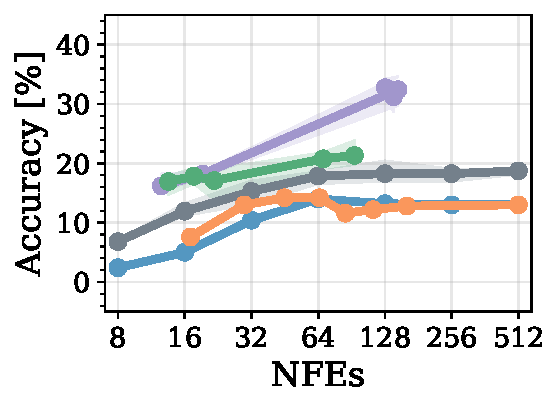
\includegraphics[width=\textwidth]{new_plots_nov4/length-transfer/bl256-to-bl512-llada-math-temp1.0.pdf}
        \caption{MATH-500}
    \end{subfigure}
    \caption{$BL=L=256$-trained policies from \Cref{sec:exp-bl256} evaluated with a 2x longer sequence length ($BL=L=512$) with $\tau_{\pi} = 1$. Note that the learned policies yield almost identical performance, while the heuristic methods degrade further compared to $L=256$ (cf. \Cref{fig:gsm8k-bl256-llada} \& \Cref{fig:math500-bl256-llada}). Both for LLaDA-8B-Instruct.}
    \label{fig:length-transfer}
\end{figure}
